\chapter{Mendix}

    \section{Τι είναι το Mendix;}
        Το Mendix είναι από τις δημοφιλέστερες πλατφόρμες ανάπτυξης λογισμικού σε low-code. Η εταιρία ιδρύθηκε στο Ρότερνταμ της Ολλανδίας το 2005 με σκοπό τη δημιουργία μιας πλατφόρμας έτσι ώστε οι επιχειρήσεις να μπορούν να αναπτύσσουν εφαρμογές γρήγορα και αποδοτικά. Το 2018 εξαγοράστηκε από τη Siemens, τη μεγαλύτερη βιομηχανική κατασκευαστική εταιρία στην Ευρώπη, κάτι που επέτρεψε να γίνουν ενσωματώσεις και βελτιώσεις σε σύντομο χρονικό διάστημα.

            \begin{figure}[h!] \noindent \centering
                    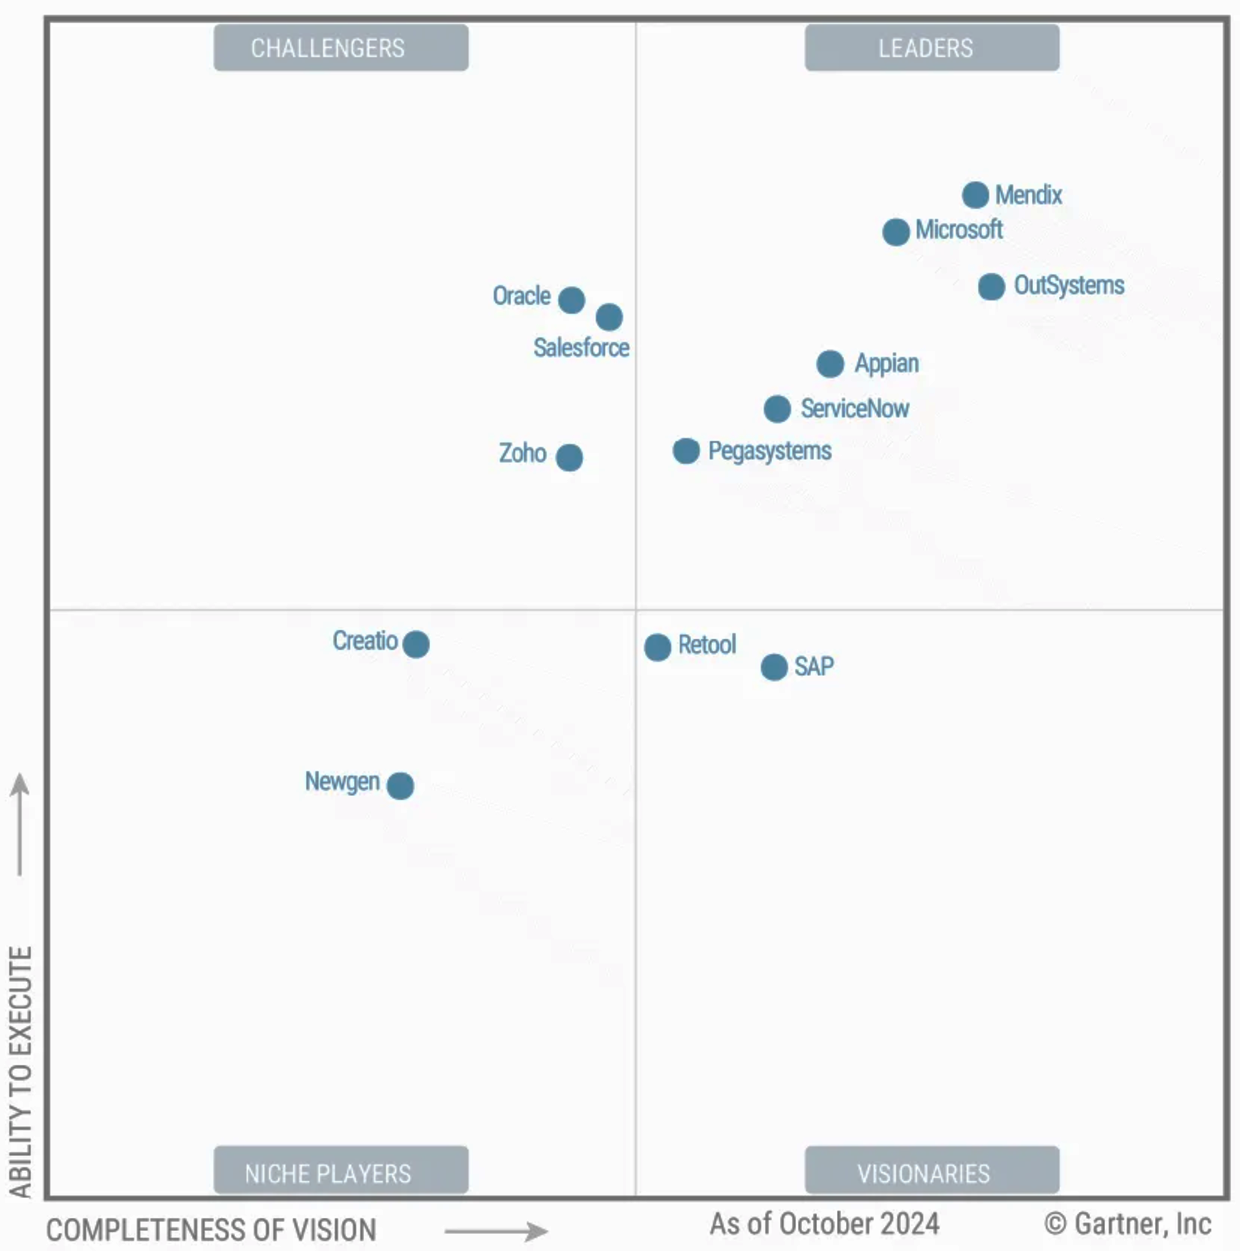
\includegraphics[width=0.5\textwidth]{GartnerQuadrant}
                    \caption{\centering Τεταρτημόριο της Gartner για πλατφόρμες ανάπτυξης λογισμικού \cite{mendixGartnerQuadrant}}
            \end{figure}

        \cite{LowCodeMendix}